We now prove the main result.
Recall that the \emph{pair} configuration consists of two dominoes which share a long side as shown in Figure \ref{fig:pair}, which can be written as
\begin{equation}
  D_\mathrm{pair} = \Big\{\{(0, 0), (1, 0)\}, \{(0, 1), (1, 1)\}\Big\}. 
\end{equation}
It turns out to be useful to consider another domino configuration, which we call a \emph{windmill}, which consists of four dominoes sharing a corner such that no two share a long side, as shown in Figure \ref{fig:windmill}. Formally, this can be written as
\begin{equation}
  D_{\mathrm{windmill}} = \Big\{\{(0, 0), (1, 0)\}, \{(0, 1), (0, 2)\}, \{(-1, 1), (-2, 1)\}, \{(-1, 0), (-1, -1)\} \Big\}.
\end{equation}
\noindent We show that the topological/graph-theoretic structure of a regular region gives a constraint on the number of these substructures contained in a given tiling. In precise terms, for a tiling $T$, we define
\begin{equation}
  \# \mathrm{pairs} (T) = |\{ S \subseteq T \mid S \cong D_{\mathrm{pair}}\}|
\end{equation}
and 
\begin{equation}
  \# \mathrm{windmills} (T) = |\{ S \subseteq T \mid S \cong D_{\mathrm{windmill}}\}|. 
\end{equation}
as the number of substructures isomorphic to the pair or the windmill, respectively.
\begin{figure}[h]
  \centering
  \begin{minipage}{0.45\textwidth}
    \centering
    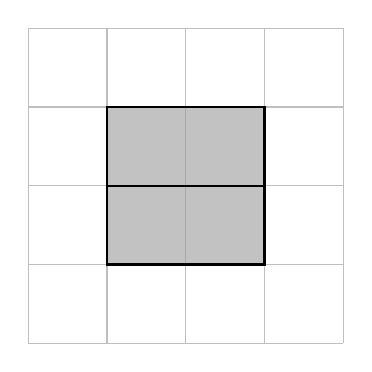
\begin{tikzpicture}
      \draw[step=1cm, black!25] (-1, -1) grid (3, 3);
      \draw[black, fill=black!40, fill opacity=0.60, thick] (0, 0) rectangle (2, 1);
      \draw[black, fill=black!40, fill opacity=0.60, thick] (0, 1) rectangle (2, 2);
    \end{tikzpicture}
    \caption{The pair configuration.}\label{fig:pair}
  \end{minipage}
  \hfill
  \begin{minipage}{0.45\textwidth}
    \centering
    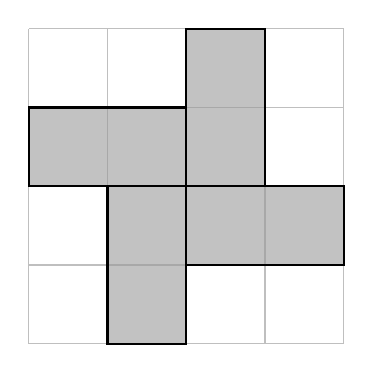
\begin{tikzpicture}
      \draw[step=1cm, black!25] (-2, -2) grid (2, 2);
      \draw[black, fill=black!40, fill opacity=0.60, thick] (0, 0) rectangle (2, -1);
      \draw[black, fill=black!40, fill opacity=0.60, thick] (0, 0) rectangle (1, 2);
      \draw[black, fill=black!40, fill opacity=0.60, thick] (0, 0) rectangle (-2, 1);
      \draw[black, fill=black!40, fill opacity=0.60, thick] (0, 0) rectangle (-1, -2);
    \end{tikzpicture}
    \caption{The windmill configuration.}\label{fig:windmill}
  \end{minipage}
\end{figure}
\begin{theorem}\label{thm:main}
  Let $R \subseteq \mathbb{Z}^2$ be a regular region. If $T$ is a domino tiling of $R$, then
  \begin{equation}
    \# \mathrm{windmills}(T) - \# \mathrm{pairs}(T) \leq b(R) - 2,
  \end{equation}
  where $b(R)$ is the number of boundary components of $R$.
\end{theorem}
\begin{proof}
  Let $\delta_T \colon R \to T$ be the map which takes a point to the unique domino containing it. Then, given a subsquare $Q \cong \{0,1\}^2$, define the \emph{divergence} of $T$ at $Q$ by
  \begin{equation}
    (\operatorname{div} T)(Q) = \frac{1}{4}\sum_{q \in Q} f(\delta_T(q); Q).
  \end{equation}
  Let $\mathcal{P}$ and $\mathcal{W}$ be the set of pairs and windmills contained in $T$, respectively. If $Q \subseteq R$ is a subsquare, then we have three cases:
  \begin{enumerate}
    \item if $Q$ is contained in an element of $\mskip 3mu \mathcal{P}$, then $\mskip 2mu (\operatorname{div} T) (Q) = -1$.
    \item if $Q$ is contained in an element of $\mathcal{W}$, then $(\operatorname{div} T) (Q) = +1$.
    \item otherwise, there is at most one domino fully contained in $Q$, so 
    \begin{equation}
      (\operatorname{div} T) (Q) = 1 - \tfrac{1}{2} \cdot|\{q \in Q \mid \delta_T(q) \subseteq Q \}| \geq 1 - \tfrac{1}{2} \cdot 1 \cdot  2 = 0.
    \end{equation}
  \end{enumerate}
  Hence, the total divergence is bounded below by the number of excess windmills, that is,
  \begin{equation}
    \sum_{Q \subseteq R} (\operatorname{div} T) (Q) \geq \#\text{windmills}(T) - \#\text{pairs}(P).
  \end{equation}
  For the rest of the argument, we calculate the sum of the divergence over each square in the region, reducing it to a sum of the \say{flux} of $\iota$ across the boundary.

  Let $q \in R$. If $q$ is an interior point, then there are exactly four subsquares $Q \cong \{0,1\}^2$ which contain it.
  Exactly two of these squares must fully contain $\delta_T(q)$, so
  \begin{equation}
    \frac{1}{4}\sum_{\substack{Q \mskip 1mu \subseteq \mskip 0.3mu R \\[0.2ex] Q \ni q}} \iota(\delta_T(q); Q) = \frac{1}{2} - \frac{1}{2} = 0.
  \end{equation}
  Otherwise, if $q$ is a boundary point, then by Lemma \ref{lem:exterior-angle},
  \begin{equation}
    \frac{1}{4}\sum_{\substack{Q \mskip 1mu \subseteq \mskip 0.3mu R \\[0.2ex] Q \ni q}} \iota(\delta_T(q); Q) \leq -\frac{\theta_{\lVert R \rVert}(q)}{2\pi}.
  \end{equation}
  Therefore, by Theorem \ref{thm:gauss-bonnet} and Corollary \ref{cor:real-components}, we have
  \begin{equation}
    \sum_{Q \subseteq R} (\operatorname{div} T)(Q) = \frac{1}{4}\sum_{q \in R} \sum_{Q \ni q} \iota(\delta_T(q); Q) \leq -\frac{1}{2\pi} \sum_{q \in \mathrm{cr}(\lVert R \rVert)} \theta_{\lVert R \rVert}(q) = b(R) - 2.
  \end{equation}
  The conclusion follows.
\end{proof}